% Source: Lecture3.pdf, page 1 (headed "Lecture 2A", rotated in the scan),
% pages 2-4 (Lecture 3); page 5 is blank.
\lecture{2A}
\subsubsection*{Pressure: high and low}

Continuation of the discussion of pressure:
\begin{equation}
  1\ \text{atm} \simeq 1\ \text{bar} = 0.1013\ \text{MPa} = 101.3\ \text{kPa}.
\end{equation}
Percy Bridgman (Harvard), in the 1920s and 1930s, achieved pressures of order
10~GPa, leading to the 1946 Nobel Prize. The DAC (diamond anvil cell) reached
$\Order(50)$--$\Order(100)$~GPa in the 1970s and 1980s; Silvera (Harvard)
$\to\Order(500\ \text{GPa})$.

Some relevant units. Torricelli: $1\ \text{torr} = 133\ \text{Pa} = 1$~mm of Hg in a
manometer (mercury is a convenient liquid to use in a manometer), and
\begin{equation}
  1\ \text{atm} = 760\ \text{mm Hg} = 760\ \text{torr} \simeq 30''\ \text{Hg}.
\end{equation}
Low pressure, vacuum conditions:
\begin{center}
\begin{tabular}{ll}
  $1$--$10^{-3}$ torr & rough vacuum\\
  $10^{-3}$--$10^{-5}$ torr & intermediate vacuum\\
  $10^{-5}$--$10^{-8}$ torr & high vacuum\\
  $10^{-8}$--$10^{-10}$ torr & very high vacuum\\
  $10^{-10}$--$10^{-12}$ torr & ultra-high vacuum
\end{tabular}
\end{center}
Applications: e.g.\ in particle physics (colliding beam machines) and studies of clean
surfaces in condensed matter physics.

\lecture{3}
\subsubsection*{Physical mechanism for liquefaction of a gas}

Next, we discuss the physical mechanism for liquefaction of a gas. Recall that the
atomic (also molecular) length scale is set by the Bohr length $a_B$:
\begin{equation}
  a_B = \frac{\hbar}{\alpha m_e c}\simeq 0.53\ \text{\AA} = 0.053\ \text{nm}.
\end{equation}
The dipole field is
\begin{equation}
  \mathbf{E}_d(\mathbf{r}) = \frac{3(\mathbf{d}\cdot\hat{\mathbf{r}})\hat{\mathbf{r}}-\mathbf{d}}{r^3},
  \qquad |\mathbf{d}|\sim e a_B,
\end{equation}
with fluctuation time scale $\sim 10^{-15}$~sec, since $\hbar\sim\Order(1)$~eV-fs.

The fluctuations in the electric charge distribution in a given atom produce a dipole
electric field $\mathbf{E}_d$ which induces a dipole moment in a neighboring atom, and
therefore there is an associated interaction energy $U$, with
$d_{\text{induced}}\sim a_B^3E_d\sim a_B^3\cdot ea_B/r^3 = ea_B^4/r^3$:
\begin{equation}
  U = -\mathbf{d}_{\text{induced}}\cdot\mathbf{E}_d
  = -\left(\frac{ea_B^4}{r^3}\right)\left(\frac{ea_B}{r^3}\right)
  = -\frac{e^2a_B^5}{r^6}\sim-\frac{e^2}{a_B}\left(\frac{a_B}{r}\right)^6
  \qquad\text{(CGS)}.
\end{equation}
This is an attraction, because the energy is negative and it gets more negative as the
distance $r$ gets smaller.

The van der Waals E.O.S.\ (equation of state) is
\begin{equation}
  \left(p + a\frac{N^2}{V^2}\right)(V-Nb) = N\kB T,\qquad \rho_n\equiv\frac{N}{V},
\end{equation}
where $Nb$ is the excluded-volume correction, $b\sim\Order(a_B^3)$. Dimensionally,
$p = F/A = E/V$, so
\begin{equation}
  \dim(a)\sim V^2\cdot\frac{E}{V} = E\cdot V\sim U_0\left\{\frac{4\pi}{3}r_0^3\right\},
\end{equation}
where $U_0$ and $r_0$ will be defined below.

This attractive interaction leads atoms (or molecules) to come closer. As the atoms (or
molecules) get so close that their electron clouds overlap, the Pauli Exclusion
Principle, which forbids identical fermions from occupying the same quantum state,
forces some electrons to move to higher-energy states, which costs energy. We can thus
deduce that the interaction energy will have a form, as a function of $r$, as shown in
the diagram.

\begin{diagram}
\begin{tikzpicture}[scale=0.9,>=Stealth]
  \draw[->] (0,0) -- (0,3.2) node[left] {$U(r)$};
  \draw[->] (0,1.2) -- (6,1.2) node[right] {$r$};
  \draw[thick,domain=1.38:5.8,samples=150,smooth]
    plot (\x,{min(3.1,1.2+1.0*((1.6/\x)^12-2*(1.6/\x)^6))});
  \draw (1.426,1.12) -- (1.426,1.28); \node[above left,font=\small] at (1.43,1.2) {$\sigma$};
  \draw[dashed] (1.6,1.2) -- (1.6,0.2); \node[below,font=\small] at (1.6,0.2) {$r_0$};
  \node[anchor=west,font=\small,align=left] at (1.9,2.8) {complicated: involves electronic wavefunctions\\
     in the atoms or molecules; can approximate as $\sim r^{-12}$};
  \node[anchor=west,font=\small] at (3.4,0.65) {$\sim -1/r^6$};
\end{tikzpicture}
\diagramcaption{The interatomic potential, with a hard core at short distance and an
attractive $r^{-6}$ tail.}
\end{diagram}

\subsubsection*{The Lennard-Jones potential}

The Lennard-Jones (6--12) energy $U(r)$ is
\begin{equation}
  U(r) = U_0\left[\left(\frac{r_0}{r}\right)^{12}-2\left(\frac{r_0}{r}\right)^{6}\right]
       \equiv 4U_0\left[\left(\frac{\sigma}{r}\right)^{12}-\left(\frac{\sigma}{r}\right)^{6}\right],
\end{equation}
with $r_0^6 = 2\sigma^6$, i.e.\ $r_0 = 2^{1/6}\sigma = 1.12\,\sigma$. The force is
$\mathbf{F} = -\boldsymbol{\nabla}U$; with $\mathbf{F} = F\hat{\mathbf{r}}$,
\begin{align}
  F &= -U_0\frac{\partial}{\partial r}\left[r_0^{12}r^{-12}-2r_0^6r^{-6}\right]
     = -U_0\left[-12r_0^{12}r^{-13}+12r_0^6r^{-7}\right]\nonumber\\
    &= \frac{12U_0}{r}\left[\left(\frac{r_0}{r}\right)^{12}-\left(\frac{r_0}{r}\right)^{6}\right];
\end{align}
$F = 0$ at $r = r_0$, the minimum of the potential.

E.g.\ Ar: $U_0/\kB = 120$~K, $r_0 = 3.8\ \text{\AA} = 0.38$~nm, with
\begin{equation*}
  T_\ell\equiv T_b = 87.5\ \text{K},\qquad T_m\equiv T_f = 84\ \text{K}
  \qquad(3.5\ \text{K difference}).
\end{equation*}
Here $T_\ell$ = liquefaction temperature $\equiv T_{\text{boil}}\equiv T_b$ and
$T_m = T_{\text{melt}}\equiv T_{\text{freeze}}$, at $p = 1$~atm.

Another example: CH$_4$ (methane). Symmetry implies $d = 0$ (no permanent electric
dipole):
\begin{equation*}
  T_\ell = T_b = 109\ \text{K},\qquad T_m = T_f = 90.7\ \text{K}.
\end{equation*}
CO$_2$ is a linear molecule; symmetry implies $d = 0$. The van der Waals analysis applies
not just to noble gas atoms (He, Ne, Ar, Kr, Xe), but more generally to atoms and
molecules (e.g.\ CH$_4$, CO$_2$) with $d = 0$.

Contrast with molecules that have permanent electric dipole moments, $d\sim ea_0$, e.g.\
H$_2$O (water), with $T_b - T_m = 100$~K, and ammonia NH$_3$. In both, the hydrogen side
carries charge $\delta+$ and the opposite side $\delta-$.

\subsection{Crystal structures and lattices}

Next, we discuss some crystal structures.

\begin{diagram}
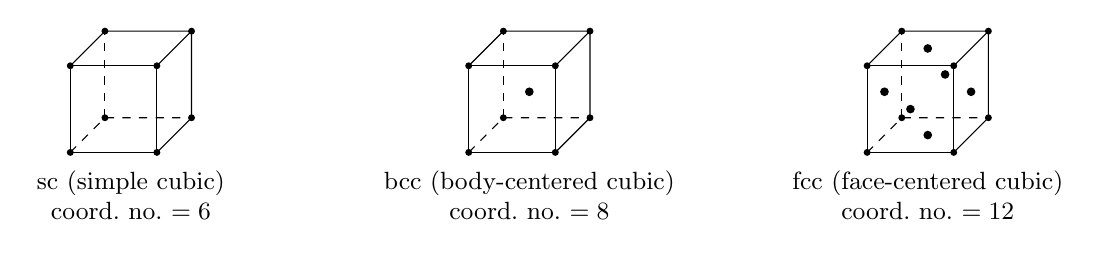
\begin{tikzpicture}[scale=1.1]
  \newcommand{\cube}{%
    \draw (0,0) rectangle (1,1);
    \draw (1,0) -- (1.4,0.4) -- (1.4,1.4) -- (1,1);
    \draw (0,1) -- (0.4,1.4) -- (1.4,1.4);
    \draw[dashed] (0,0) -- (0.4,0.4) -- (1.4,0.4);
    \draw[dashed] (0.4,0.4) -- (0.4,1.4);
    \foreach \p in {(0,0),(1,0),(0,1),(1,1),(0.4,0.4),(1.4,0.4),(0.4,1.4),(1.4,1.4)} \fill \p circle (0.04);}
  \begin{scope}\cube \node[below,align=center,font=\small] at (0.7,-0.1) {sc (simple cubic)\\ coord.\ no.\ $=6$}; \end{scope}
  \begin{scope}[xshift=4.6cm]\cube \fill (0.7,0.7) circle (0.05);
    \node[below,align=center,font=\small] at (0.7,-0.1) {bcc (body-centered cubic)\\ coord.\ no.\ $=8$}; \end{scope}
  \begin{scope}[xshift=9.2cm]\cube
    \foreach \p in {(0.5,0.5),(0.9,0.9),(0.7,0.2),(0.7,1.2),(0.2,0.7),(1.2,0.7)} \fill \p circle (0.05);
    \node[below,align=center,font=\small] at (0.7,-0.1) {fcc (face-centered cubic)\\ coord.\ no.\ $=12$}; \end{scope}
\end{tikzpicture}
\diagramcaption{Cubic lattices.}\label{fig:cubic}
\end{diagram}

The sc (simple cubic) lattice has coordination number 6. The coordination number of a
general $\mathbb{Z}^d$ lattice is $2d$. The coordination number of the bcc
(body-centered cubic) lattice is 8, and that of the fcc (face-centered cubic) lattice is
12.

Two-dimensional lattices:
\begin{itemize}
  \item square lattice, coordination number 4, denoted $4^4$. The square lattice is
    bipartite: $\Lambda_{sq} = \Lambda_e\oplus\Lambda_o$ (even, odd). More generally
    $\Lambda = \bigoplus_i\Lambda_i$.
  \item triangular (tri) lattice, coordination number 6, denoted $3^6$.
  \item honeycomb (hc) = hexagonal lattice, coordination number 3, denoted $6^3$; also
    bipartite, $\Lambda_{hc} = \Lambda_e\oplus\Lambda_o$.
\end{itemize}
These are the total set of homopolygonal 2D lattices.

The duality transformation $\Lambda\leftrightarrow\Lambda^*$ maps a face of $\Lambda$ to a
vertex on $\Lambda^*$, and hence a vertex on $\Lambda$ to a face on $\Lambda^*$; the bonds on
$\Lambda^*$ connect vertices in $\Lambda^*$.

\begin{diagram}
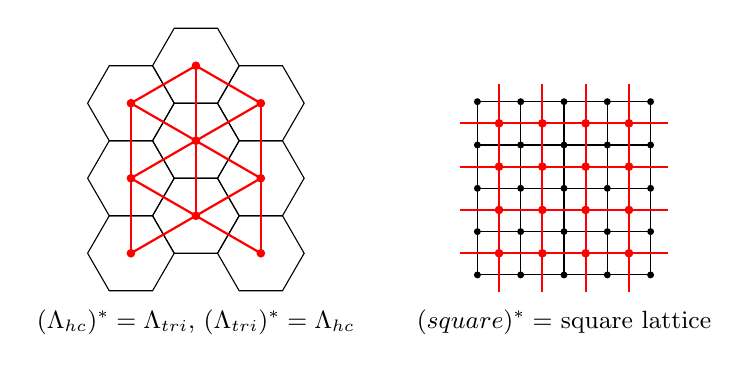
\begin{tikzpicture}[scale=0.55]
  % honeycomb with its dual triangular lattice
  \foreach \i in {0,1,2} \foreach \j in {0,1,2} {
    \pgfmathsetmacro{\cx}{1.5*\i}
    \pgfmathsetmacro{\cy}{sqrt(3)*\j + mod(\i,2)*sqrt(3)/2}
    \draw (\cx,\cy) +(0:1) -- +(60:1) -- +(120:1) -- +(180:1) -- +(240:1) -- +(300:1) -- cycle;
  }
  \foreach \i in {0,1,2} \foreach \j in {0,1,2} {
    \pgfmathsetmacro{\cx}{1.5*\i}
    \pgfmathsetmacro{\cy}{sqrt(3)*\j + mod(\i,2)*sqrt(3)/2}
    \fill[red] (\cx,\cy) circle (0.1);
  }
  \draw[red,thick] (0,0) -- (0,{sqrt(3)}) -- (0,{2*sqrt(3)});
  \draw[red,thick] (3,0) -- (3,{sqrt(3)}) -- (3,{2*sqrt(3)});
  \draw[red,thick] (1.5,{sqrt(3)/2}) -- (1.5,{3*sqrt(3)/2}) -- (1.5,{5*sqrt(3)/2});
  \draw[red,thick] (0,0) -- (1.5,{sqrt(3)/2}) -- (3,0);
  \draw[red,thick] (0,{sqrt(3)}) -- (1.5,{3*sqrt(3)/2}) -- (3,{sqrt(3)});
  \draw[red,thick] (0,{2*sqrt(3)}) -- (1.5,{5*sqrt(3)/2}) -- (3,{2*sqrt(3)});
  \draw[red,thick] (0,{sqrt(3)}) -- (1.5,{sqrt(3)/2}) -- (3,{sqrt(3)});
  \draw[red,thick] (0,{2*sqrt(3)}) -- (1.5,{3*sqrt(3)/2}) -- (3,{2*sqrt(3)});
  \node[font=\small] at (1.5,-1.6) {$(\Lambda_{hc})^* = \Lambda_{tri}$, $(\Lambda_{tri})^* = \Lambda_{hc}$};
  % square lattice and its dual
  \begin{scope}[xshift=8cm,yshift=-0.5cm]
    \foreach \x in {0,...,4} \draw (\x,0) -- (\x,4);
    \foreach \y in {0,...,4} \draw (0,\y) -- (4,\y);
    \foreach \x in {0,...,4} \foreach \y in {0,...,4} \fill (\x,\y) circle (0.08);
    \foreach \x in {0.5,1.5,2.5,3.5} \draw[red,thick] (\x,-0.4) -- (\x,4.4);
    \foreach \y in {0.5,1.5,2.5,3.5} \draw[red,thick] (-0.4,\y) -- (4.4,\y);
    \foreach \x in {0.5,1.5,2.5,3.5} \foreach \y in {0.5,1.5,2.5,3.5} \fill[red] (\x,\y) circle (0.1);
    \node[font=\small] at (2,-1.1) {$(\text{square})^* = $ square lattice};
  \end{scope}
\end{tikzpicture}
\diagramcaption{Duality transformation between the honeycomb and triangular lattices
(left), and the self-duality of the square lattice (right). The dual lattice is drawn
in red.}\label{fig:duality}
\end{diagram}

So the square lattice is self-dual.

There are also regular lattices composed of more than a single type of regular polygon;
these are called heteropolygonal. Example: the $4\cdot 8\cdot 8 = 4\cdot 8^2$
(``bathroom tile'') lattice.

\begin{diagram}
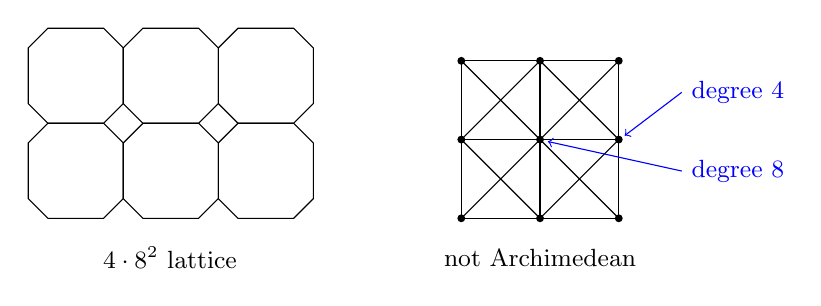
\begin{tikzpicture}[scale=0.5]
  \pgfmathsetmacro{\s}{1/(1+sqrt(2))}
  \foreach \i in {0,1,2} \foreach \j in {0,1} {
    \begin{scope}[shift={(2.414*\i,2.414*\j)}]
      \draw (0.5,0) -- (1.914,0) -- (2.414,0.5) -- (2.414,1.914) -- (1.914,2.414) -- (0.5,2.414) -- (0,1.914) -- (0,0.5) -- cycle;
    \end{scope}}
  \node[font=\small] at (3.6,-1) {$4\cdot 8^2$ lattice};
  \begin{scope}[xshift=11cm]
    \draw (0,0) rectangle (4,4);
    \draw (2,0) -- (2,4); \draw (0,2) -- (4,2);
    \draw (0,0) -- (4,4); \draw (0,4) -- (4,0);
    \draw (0,2) -- (2,4) -- (4,2) -- (2,0) -- cycle;
    \foreach \x in {0,2,4} \foreach \y in {0,2,4} \fill (\x,\y) circle (0.1);
    \draw[->,blue] (5.6,3.2) -- (4.15,2.1); \node[anchor=west,blue,font=\small] at (5.6,3.2) {degree 4};
    \draw[->,blue] (5.6,1.2) -- (2.2,1.95); \node[anchor=west,blue,font=\small] at (5.6,1.2) {degree 8};
    \node[font=\small] at (2,-1) {not Archimedean};
  \end{scope}
\end{tikzpicture}
\diagramcaption{Left: the heteropolygonal $4\cdot 8^2$ (``bathroom tile'') lattice.
Right: an example of a planar lattice that is not Archimedean, since some vertices
have degree 4 and others degree 8.}\label{fig:488}
\end{diagram}

Definition: an \emph{Archimedean lattice} is a regular tiling of the plane with some set
of regular polygons such that every vertex is equivalent to every other vertex.

Synonymous terms (math = physics): vertex = site; edge = bond.

Definition: the \emph{degree} of a vertex is the number of edges (= bonds) connecting to
it.
